\documentclass[../main.tex]{subfiles}

\begin{document}
\section{Targeting and Combat}
This section explains the rules for targeting units and resolving combat.

\subsection{Targeting a Unit}
The following rules apply for any action or skill that requires a unit to be targeted, not just the Attack Action.

When an action or skill requires a target to be selected, check to make sure the targeted unit is within the range specified by the skill or action. Then, check to make sure the targeted unit is within line of sight of the unit using the skill or performing the action.

\textit{Exception: Units that are engaged with each other or are both on the Sentience may always target each other, even if they do not have line of sight to each other.}

\subsubsection{Line of Sight}
Line of sight is used to determine whether one unit can “see” another unit. Establishing line of sight is required when attempting to target a unit, unless a skill or item specifies otherwise. Unlike range, the line of sight is a straight line drawn between the targeted unit’s hit box and the vision point of the unit that is selecting a target. Line of sight is unrelated to the number of hexes between two units.

The red dot is the vision point, the black coloring is not targetable, the light gray is targetable.

\begin{figure}[h]
    \centering
    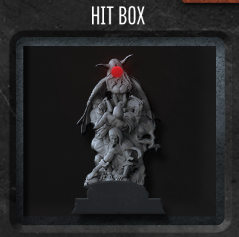
\includegraphics[width=0.75\linewidth]{chapters//TargetingandCombat/TimeStrikeHitBox.png}
\end{figure}

\textit{Image: Hit Box}

\subsubsection{How to Determine Line of Sight}
\begin{enumerate}
    \item Check the vision point (the green dot on the targeting unit’s Character card) and the hit box (The red area on the targeted unit’s Character card) of the two units.
    \item Stand behind the targeting unit to see if its vision point can “see” any part of the targeted unit’s Hit Box.
    \item If an unobstructed straight line can be drawn between the targeting unit’s vision point and the targeted unit’s hit box, then the targeting unit has line of sight to the targeted unit.
\end{enumerate}

\textit{Example: If a unit is attempting to target a unit around a wall or obstacle and only part of the targeted unit is visible, this is a good time to check for line of sight.}

\begin{figure}[h]
    \centering
    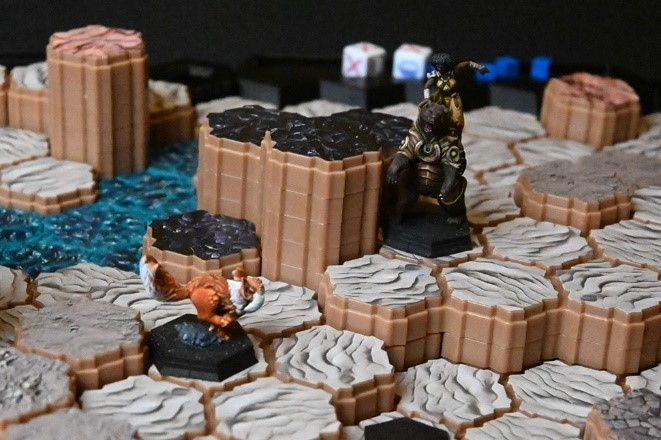
\includegraphics[width=1\linewidth]{chapters//TargetingandCombat/TimeStrikeLineofSight.jpg}
\end{figure}

\textit{Image: Successful line of sight.}


\begin{figure}[h]
    \centering
    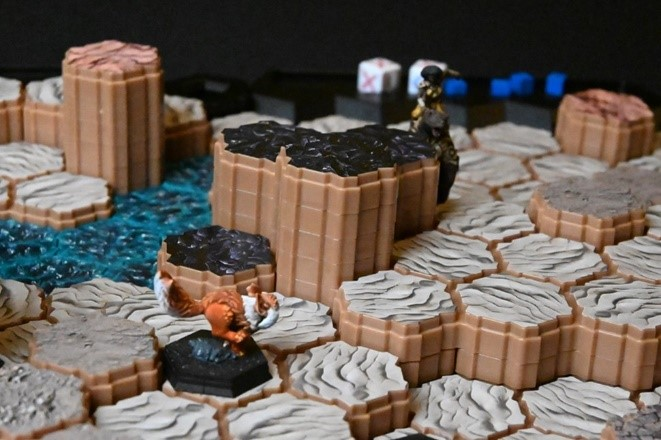
\includegraphics[width=1\linewidth]{chapters//TargetingandCombat/TimeStrikenotlineofsight.jpg}
\end{figure}
\textit{Image: Obstructed line of sight.}

\textit{Recommendation: If it is difficult to determine whether a unit has line of sight to their target, use a string or rubber band to attempt connecting the targeting unit’s vision point to the hit box of the targeted unit with a straight line. If the string cannot connect the two points with a straight line, then line of sight is not established.}



\subsubsection{Targeting through other Units}

A unit may attempt to target another unit even if there are other units between them, but the targeting unit must still have a clear line of sight to their target. If the unit(s) between the targeting unit and the targeted unit fully obstruct the line of sight, then the targeting unit is unable to successfully target the unit.

\subsection{Attacking a Unit}
If another unit is within range and line of sight of a player’s unit during their activation, the active unit may use 1 Energy to select a target and perform the Attack Action.
\begin{enumerate}
    \item Select a unit as a target for the attack. When performing the Attack Action, the targeted unit must be no further away than the attacking unit’s Range stat. \textit{(Remember that if a unit is engaged, it may only target units that it is engaged with when performing an Attack Action).}
    \item Calculate the total Attack stat by checking the Attack stat on the Character card as well as any modifiers incurred by height advantage, buffs, curses, or equipped loot.
    \item Roll a number of D6 equal to the attacker’s total Attack stat.
    \item Each rolled Attack icon will count as one hit against the target.
    \item After performing the Attack Action, the active unit may no longer use their Movement or use their Energy to take additional actions for the remainder of the turn.
\end{enumerate}

\textit{Note: Be sure to check for Lucky Attack sides, since Characters can trigger special effects from Lucky rolls.}
\begin{figure}[h]
    \centering
    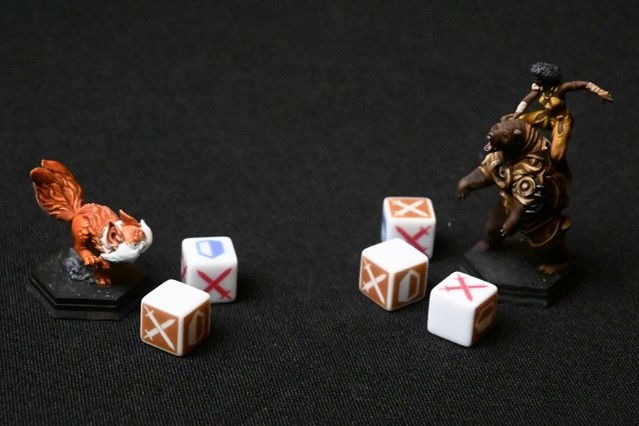
\includegraphics[width=1\linewidth]{chapters//TargetingandCombat/TimeStrikeAttacking.jpg} 
\end{figure}

\textit{Image: (Right) A unit attacking an enemy with 3 dice and rolling 2 Attack icons. (Left) A unit defending itself with 2 dice and rolling 1 Defense icon. }

\subsection{Area of Effect}
Certain skills may cause attacks to affect multiple hexes or multiple units. In this case, the attacker still only rolls for the attack once, and each unit that is affected by the attack rolls defense individually, in an order chosen by the attacking player.

\subsection{Defending Against an Attack}
When a unit is attacked by another unit, it can defend itself from the attack.

\subsubsection{How to Defend?}
\begin{enumerate}
    \item Calculate the total Defense stat by checking the Defense stat on the Character card as well as any modifiers incurred by height advantage, buffs, curses, or equipped loot.
    \item Roll a number of D6 equal to the defender’s total Defense stat.
    \item Each rolled Defense icon will count as one block against a hit from the attacker.
    \item For each hit that was not blocked, place a marker in the Health Bar of the defending unit. 
\end{enumerate}

\textit{Note: Be sure to check for Defense skills on the Character that can be used.}

\begin{figure}[h]
    \centering
    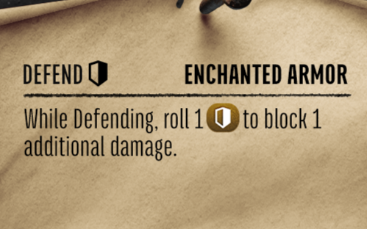
\includegraphics[width=0.5\linewidth]{chapters//TargetingandCombat/TimeStrikeDefenseSkills.png}
\end{figure}

\textit{Image: Defense skill that requires a Lucky Defense roll to activate.}

\subsection{Height Advantage}
If one unit is on a higher hex than another unit, it is considered to have height advantage against that unit. Height advantage allows the unit to have an increased total Attack or total Defense stat while attacking or defending.

\subsubsection{How to use height advantage?}
If a unit is attacking another unit from height (its base is higher than the base of the unit it is targeting), the attacking unit adds +1 when calculating its total Attack stat.

If a unit is defending against an attack and its base is higher than the attacker’s, the defending unit adds +1 when calculating its total Defense stat.

\begin{figure}[h]
    \centering
    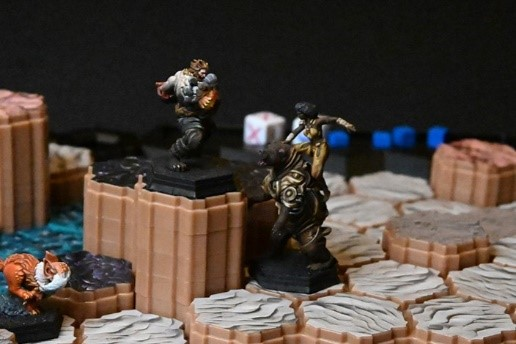
\includegraphics[width=0.75\linewidth]{chapters//TargetingandCombat/TimeStrikeHeightAdvantage.jpg}
\end{figure}

\textit{Image: Two Characters battling with one having height advantage.}

\subsection{Melee Units}
A unit with a Range stat of 1 is a Melee unit, which will be listed next to the Range stat on its Character card. A Melee unit can only attack units that it is engaged with. The Range stat of Melee units cannot be modified.

\textit{Note: Melee units may still have ranged skills that can be used against non-adjacent enemies.}

\subsection{Jump Attack}
Jump Attacks allow Melee units to increase their attack range by leaping through the air to come smashing down on their targets below.

\subsubsection{How to Jump Attack? }
If a Melee unit is unengaged and has at least 1 unused Energy during its activation, it may target an enemy unit within 2 range whose base is on a lower hex than the Melee unit and perform a Jump Attack against it.

\begin{enumerate}
    \item Place the Melee unit on the nearest unoccupied hex adjacent to its target so that the two units are engaged.
    \item Use 1 Energy to perform an Attack Action against the targeted unit. During this attack, the attacking unit is always considered to have height advantage.
    \item After resolving the attack, if the difference in height between the attacker’s original position and the hex that it landed on is greater than the attacker’s Height stat, the attacker must roll for fall damage.
\end{enumerate}

\textit{Note: All movement type units are subjected to fall damage when jump attacking. However, landing in water still negates fall damage during jump attacks.}

\begin{figure}[h]
    \centering
    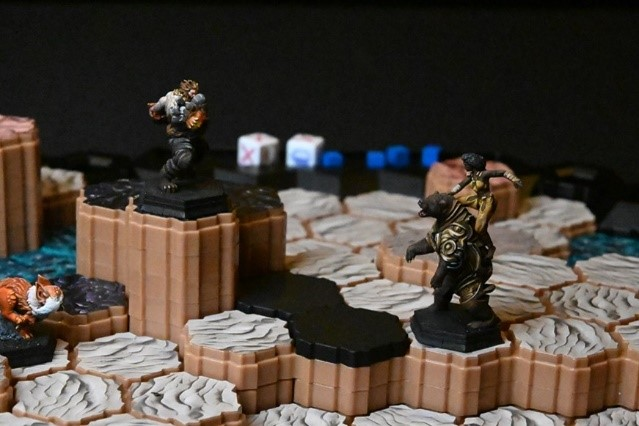
\includegraphics[width=1\linewidth]{chapters//TargetingandCombat/TimeStrikeJumpAttack1.jpg}
\end{figure}
\textit{Image: Character getting ready to Jump Attack a unit and jumping 2 hexes.}

\begin{figure}[h]
    \centering
    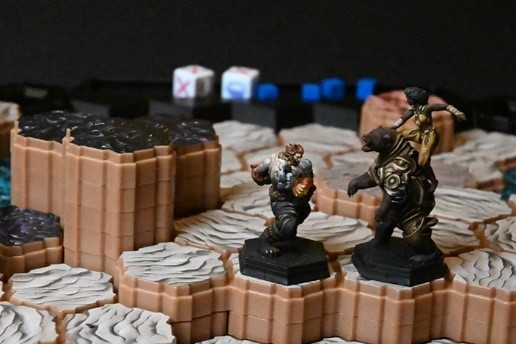
\includegraphics[width=1\linewidth]{chapters//TargetingandCombat/TimeStrikeJumpAttack2.jpg}
\end{figure}
\textit{Image: Character landing after the Jump Attack}

\textit{Note: A character can land lower or higher than their target when performing a jump attack but they must be engaged when landing. Otherwise they are landing too low or high.}

\subsection{Defeating a Unit or Character}
A unit is defeated when the number of markers in its Health Bar is equal to that unit’s maximum health. Remove defeated units from the board.

A Character is defeated when all units belonging to the Character have been defeated.

\subsubsection{Steps to take when a Character is defeated:}
\begin{enumerate}
    \item If the Character was defeated by an attack, ability skill, or Cheap Shot, any goods in the defeated Character’s inventory are transferred to the inventory of the Character that defeated them.
    \item Remove the defeated Character from the board.
\end{enumerate}
\textit{Note: If a Character is defeated by the Lost their goods are discarded.}

\subsection{Multiple Attacks}

Some units may have skills, items, or other scenarios that let them use the Attack action more than once. In this case, after they use their first Attack, they cannot move but they can use their remaining energy to Attack again.

\clearpage

\end{document}